\documentclass[conference]{IEEEtran}
\ifCLASSINFOpdf
\else
\fi
\hyphenation{op-tical net-works semi-conduc-tor}
\usepackage{graphicx}
\begin{document}
\title{Notification Center}
\author{\IEEEauthorblockN{Mihai Ciorobea}
\IEEEauthorblockA{Ingineria sistemelor Internet\\
Universitate Politehnica Bucuresti\\
Email: mihai.ciorobea@cti.pub.ro}}
\maketitle
\begin{abstract}
In secolul XXI, cand orice om, ca este mai tanar sau mai invarsta, ca este mai in ton cu tehnologia sau este mai clasic, cu totii avem multe lucruri pe cap. Cu toti avem nevoie de  ceva, care sa ne aduca aminte de toate lucrurile pe care trebuie sa le facem zi de zi. Fie ca acel ceva se numeste o foaie fie ca se numeste un telefon, cu totii avem nevoie de el.

Astfel ne propunem sa facem o aplicatie care sa ajute orice utilizator sa isi creeze o lista de alerte care sa il ajute pe acesta sa isi reaminteasca orice sarcina pe care acesta o are de indeplimit.
\end{abstract}
\IEEEpeerreviewmaketitle
\section{Introducere}
In viata de zi cu zi avem multe lucruri de facut. O zi normala a unuia dintre noi poate sa contina si pana la 20 sau chiar 30 de lucruri de facut, cum ar fi: 
\begin{itemize}
  \item mers la serviciu
  \item cumparaturi
  \item spalat masina
  \item luat copilul de la scoala
  \item dus gunoiul
  \item etc\ldots
\end{itemize}

Pentru multe din acestea nu avem nevoie de cineva sa ne reaminteasca sa le facem, pentru ca sunt sarcini de zi cu zi. In mare aceste lucruri sunt acele sarcini pe care daca nu le facem se poate observa usor lipsa lor. Cel mai simplu si mai intuitiv exemplu este cel al  mancatului. Dupa cum stim, multi oameni atunci cand sunt prinsi cu ceva foate interesant si captivant, uita sa mai manance. In acele momente organismul nostrul este cel care aduce aminte fiecaruia dintre noi ca a uitat ceva. 

Exact cum organismul este in cazul mancarii, asa in diferite cazuri exista alte metode de a reaminti lucruri pe care trebuie sa le faci. Pana acum am vorbit de sarcini care le avem de facut zi de zi, dar in cazul celor care sunt mai rare ? Unul din cele mai utilizate exemple este acela al facturilor la energie, gaze, etc. Acestea sunt deja urmatorul nivel de sarnici, sarcini ce au o frecventa mai mica dar poate au o importanta mai mare. Poate extrapoland putin putem ajunge la sarnici cu o frecventa mult mai mica, cum ar fi impozitul sau alte plati anuale sau chiar mai rare.

Fiecare din noi avem nevoie de cineva sau de ceva care sa ne aduca aminte sa facem toate sarcinile, fie ele mici fie mari, fie foarte frecvente fie foarte rari sau poate de cele mai neimportante dar care fac totusi diferenta.

Acum ca am identificat o posibila problema cu care multi dintre noi ne confruntam, haideti sa o elaboram putin mai bine. In general chiar daca este mai in ton cu tehnologia sau nu, toate lumea trebuie sa isi noteze lucrurile care le are de facut pe o perioada viitoare fie ea scurta fie lunga. Cu alte cuvinte cu totii avem nevoie de o lista de sarcini.

In zilele noastre s-au inventat multe dispozitive care te ajuta sa faci si sa iti amintesti aproape orice, fie cu ajutorul unei varietati foarte mare de aplicatii fie doar cu ajutorul puterii sale uriase de calcul care poate incapea chiar si buzunar, intr-un telefon, dar chiar si in ceasul de mana. Toate aceste dispozitive sau programe ne sunt de mare folos, iar cu ajutorul lor viata noastra a devenit putin mai usoara, cel putin in privinta unor lucruri.





\section{Solutii similare}

In zilele noastre exista multe aplicatii care te pot ajuta sa nu uiti lucruri. Aceste aplicatii au multe denumuri posibile:
\begin{itemize}
  \item TO-DO apps
  \item Reminder apps
  \item etc\ldots
\end{itemize}

Aplicatii asemanatoare exista si sunt oferite chiar de companii mari care fac diferenta. Spre exemplu GOOGLE ofera o functionalitate asemanatoare in Google Tasks. Aceasta aplicatie vine si ca extensie oficiala de Chrome cat si ca serviciu sau utilitar. Este usor de folosit are prescutari cum ar fi: 't' pentru a adauga rapid o sarcica. Are deasemenea si posibilitatea de a vedea lista de taskuri cat si cele care au facut facute deja. Alta posibilitate de a adauga rapid task-uri este de a selecta un text din orice pagina web si de a adauga rapid acel text ca si sarcica. Task-urile sunt vizibile peste tot, ca utilizatorul sa le vada cat mai usor: 
\begin{itemize}
  \item Gmail
  \item Google Calendar
  \item iGoogle
  \item Mobile
  \item Google Tasks API
\end{itemize}

Toate aceste locuri sunt posibile aplicatii care permit utilizatoruilui sa aduge sarcini si sa isi reaminteasca ce alte lucruri mai are de facut. 

Deasemenea extensia de Chome este realizata ca exemplu pentu folosirea API-urilor expuse de Google pentru Google Tasks, iar ce care vor sa contribuie pot contribui sau isi pot dezvolta propria idee pe baza lor.

Deasemenea Apple a introdus o aplicatie numita Notification Center in iOS cat si in OS X. Aceaste aplicatie ofeara o vedere generata asupra toturor alertelor celorlalte aplicatii. Arata notificarile pana cant utilizatorul le marcheaza ca si complete. Utilizatorii pot alege care aplicatii sa apara in Notification Center si cum sa le utilizeze. 




Notification Center a fost lansat în iOS 5 pentru a inlocui sistemul anterior de a face cu împingere și notificări locale. În loc de a întrerupe utilizatorul cu o alertă, Notification Center afișează în schimb un banner in partea de sus a ecranului. Acest lucru permite utilizatorului de a continua utilizarea dispozitivului lor, și dispare după o anumită perioadă de timp. Toate notificările anterioare sunt adunate în panoul de Notification Center, care pot fi afișate în iOS prin glisarea în jos de pe bara de stare, și în OS X, făcând clic pe butonul central de notificare (sau folosind gesturi track - pad, trecând de la dreapta la stânga). Notificările pot fi selectate de către utilizator, care redirecționează utilizatorul la cererea în cazul în care notificarea a fost creat inițial, și că marcajul alertei ca fiind citite. Odată ce o notificarea este citita, acesta este eliminata din panoul. Utilizatorii pot elimina, de asemenea, notificări, fără a le citi prin ștergerea alerte individuale, sau de respingere toate alertele unei aplicații din cadrul aplicației, care este generatoare de ele. Când un dispozitiv iOS este blocat, noi notificări apar pe ecranul de blocare, iar utilizatorii pot accesa aplicația trecând pictograma aplicației cu degetul de la stânga la dreapta de-a lungul notificării.
Centrul de notificare pe iPhone și iPod Touch include, de asemenea, starea vremii și a stocurilor de widget-uri, afișarea de informații cu privire la vremea în locația curentă a utilizatorului, precum și orice stocuri care utilizatorul a selectat în aplicația Stocuri. Această caracteristică nu este disponibilă pe iPad sau OS X. Utilizatorii pot selecta, de asemenea, opțiunea de a afișa butoanele de Twitter și Facebook, permițându-le pentru a trimite tweet-uri sau să actualizeze statusul direct de la notificare Center.
Orice aplicație care utilizează sistemul de Notificari Push furnizate de Apple, sau notificări locale, se poate utiliza de notificare Center. Utilizatorii pot personaliza ceea ce doresc să apară în Notification Center, și pot opta pentru a opri anumite aplicații care apar în Notification Center, sau trimiterea alerte la ecranul lor. Utilizatorii OS X se poate dezactiva, de asemenea, alerte și bannere pentru o zi, oprind notificări care apar pe ecran. Cu toate acestea, orice notificări trimise în acest timp sunt încă vizibile în panoul de Notification Center. Un serviciu similar este inclus în iOS 6, ca parte din caracteristica 'Do Not Disturb'.


Desigur exista aplicatii asemanatoare realizate de companii nu atat de cunoscute cat Google sau Apple. Unul din exemple este aplicatia Life Reminders realizata de Cameleo-tech. Folosing Life Reminders se pot crea usor sarcini de zi cu zi si apoi sa uiti de toate. Cand timpul vine aplicatia o sa iti reaminteasca ea. Folosind Life Reminders, poti crea usor urmatoarele alerte:
\begin{itemize}
  \item Telefoane: utilizatorul ii specifica aplicatiei pe cine trebuie sa sune, ora si data si apoi cand este cazul este notificat si tot ce trebuie sa faca e sa dai click.. sau acesta are posibilitatea de amana actiunea. 
  \item Task-uri: tot ce trebuie adaugat este descrierea cat si data, apoi cand este cazul utilizatorul este notificat
  \item SMS/EMAIL: trebuie introduse textul cat si contactul cui i se adreseaza, iar cand este cazul mesajul poate fi trimis automat sau se asteapta o confirmare.
\end{itemize}
Compania care a creat aceasta aplicatie este chiar dispusa sa adauge noi functionalitati pe baza cerintelor clientilor. Conform specificatiilor lor, cu ajutorul unui email oricine ii poate contacta pentru  sugestii sau pentru orice problema tehnica sau non-tehnica.

\section{Arhitectura}


In conformitate cele prezentate mai sus, aplicatia noastra numita Notification Center, o sa puna la dispozitia utilizatorilor posibilitatea de a-si seta alerte si de a fi notificati cand acestea expira.

Desi exista o variatate de aplicatii care iti ofera posibilitatea de a crea alerte si de a-ti mentine o lista de sarcini pe care utilizatorul le are de indeplinit, aproape nici macar una din aceste toate aplicatii nu ofera posibilitatea de a crea liste de task-uri distribuide intre utilizatori, cat si alerte customizabile.

\subsection{Alegerea functionalitatiilor}
Dupa cum se stie in domeniul IT, din varietatea de functionalitati posibile nu se realizeaza toate. Motivul principal este calitatea. Poti creea un produs complet care sa nu mearga, sau sa nu fie utilizabil in mare masura. De asemenea poti crea o aplicatie cat de cat completa dar in care sa nu ai incredere completa si desigur exista mareu posibilitatea sa incluzi in aplicatia dorita doar functionalitatile de care esti sigur de-antregul. De aceea aplicatie realizata de noi, are si functionalitati existente la alte aplicatii cat si lucruri noi.

In multitudirea de functionalitati posibile pentru o astfel de aplicatie, Notification Center pune la dispozitie:
\begin{itemize}
  \item Crearea unui eveniment
  \item Specificarea date/orei in cadrui evenimentului creat
  \item Transformarea unui eveniment intr-o notificare
  \item Posibilitatea de a crea grupuri de utilziatori
  \item Posibilitatea setarii unui status atasat unei alerte
  \begin{itemize}
  	\item Pending
  	\item InProgress - by user
  	\item Done
  	\item NotDone
  \end{itemize}

  \item Posibilitatea de a fi notificat in mai multe feluri
  \begin{itemize}
  	\item Email
  	\item SMS
  	\item Phone
  \end{itemize}
\end{itemize}

\subsection{Detalii de implementare}

In cadrul aplicatiei Notification Center, utilizatorii isi vor seta multiple alerte care sa ii notifice la expirarea termenului limita. Asftel la o prima vedere aplicatie se incadreaza foarte repede in cadetoria Big Data, NoSQL.

In cadrul acestei abordari ar exista o baza de date nerelationala in care se afla toate datele la care aplicatia noastra ar trebui sa notifice pe cineva. Astfel aplicatia noastra ar avea o baza distribuita nerelationala in care ar tine toate alertele tuturor utilizatorilor. 

De ce ar parea ca am avea nevoie de o baza de date nerelationala ? Cel mai potrivit raspuns este: cresterea numarului de utilizatori si de alerte ale acestora. Pentru fiecare utilizator existent, sigur o sa existe relativ destul de multe intrati in tabela de alerte. 

Sa consideram ca am avea o crestere de utilizatori de 7\% pe luna, asta ar insemna ca exact in 10 luni numarul de utilizatori s-ar dubla. Considerand de asemenea ca exista o crestere de doar 7\% in numarul de alerte per utilizator, asta ar insemna ca in doar 10 luni calendaristice dimensiunea bazei noastre de date s-ar mari de 4 ori. Iar daca luam in considerare ca in general se doresc cresteri care uneori depasesc chiar si 100\%, este clar ca avem nevoie de ceva care sa scaleze si sa scaleze fara costuri considerabile.


Cu toate acestea s-a ales alegerea unei baze de date relationale. Motivul principal este acela ca in urma unor analize amanuntite, se pare de baza de date a aplicatiei Notification Center o sa aibe peste 90\% citiri pentru alerte. In cadrul citirilor din baza de date, nu sunt luate in rezultat decat primele alerte sortate cronologic. Astfel cea mai buna alegere pare cea a unei baze de date nerelationala.

Aplicatia noastra are 2 componente importante:
  \begin{itemize}
  	\item Aplicatie web - aceaste parte este include la randul ei
      \begin{itemize}
        \item partea HTML
        \item partea de server
      \end{itemize}
  	\item Cronul - care se ocupa de partea de notificari
  \end{itemize}
  
Fiecare componenta este importanta in felul ei si fiecare are rolul ei bine stabilit

\subsubsection{Aplicatia Web}

Este cea care serveste contenul HTML impreuna cu CSS-ul cat si cu JavaScript-ul atasat. Pe langa partea de Web, aceasta componenta se ocupa de toata logica de server cat si de toate securitatea aplicatiei.

Atat serverul cat si clientul au ca si protocol de transmitere a detelor in format usor de citit -- JSON (JavaScript Object Notation)

\begin{figure}[ht!]
\centering
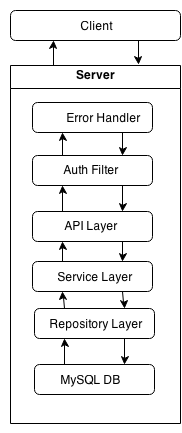
\includegraphics[height=90mm]{arhitecture.png}
\caption{Arhitectura aplicatiei}
\label{overflow}
\end{figure}

Pentru realizarea acestei componente, a fost realizata folosind librarii pentru diferite scopuri. A fost folosit pachetul de persistence de la javax cat si	libraria de hibernate, amandoua pentru realizarea legaturii cu baza de date. Peste aceste 2 librari s-a realizat un model format din entitati care modeleaza tabelele bazei de date.

De asemenea module de spring au fost folosite. Dintre care reamintim:
\begin{itemize}
        \item spring-context
        \item spring-webmvc
        \item spring-web
        \item spring-security-web
        \item spring-security-config
        \item spring-test
      \end{itemize}
Modulele de spring au fost alese in favoare modulului de JAR-RX 2.0 pentru usurinta injectarii de obiecte cat si usurinta de creare de API-uri. 

Desigur pentru accesul neautorizat folosim un filtru de autorizare. Aceste nu lasa sa treaca decat cererile care au fost autentificare si autorizare.

Pentru mentinerea autentificarii folosim user session cu context injection. Aceste este chivalent unui cookie http dar defapt inseamna autentificarea utilizatorului curent.
      
Dupa cum se poate observa in figura 1, exista mai multe componente ale aplicatiei, care puse cap la cap creaza intreaga aplicatie. Clientul trimite cereri HTTP de tip GET sau POST care ajung la server. Acesta cerere este luata de modului de Spring care are un submodul de tratare de errori. Astfel orice eroare aparuta in aplicatia noastra nu va fi vizibila direct utilizatorului, fiind prinza initial de acest modul de errori.

Dupa ce cererea a trecut de modulul de management de erori, acesta ajunge in modulul de validare a autorizarii si autentificarii. Acest modul lasa sa treaca doar cererile care au dreptul sa treaca mai departe. Desigur exceptie fac cererile de autorizare care nu sunt interceptate de acest modul.

Abia acum cererea ajunge efectiv la partea din server care o va rezolva si ii va intoarce rezultatul. Dupa cum se poate observa in figura, exista si aici mai multe nivele arhitecturale. Exista nivelul de API-uri, care vorbeste doar cu cel de servicii. La randul sau nivelul de servicii se afla intre cel de API-uri cat si cel de Repository. Acest ultim nivel este cel care face legatura directa cu baza de date.

Baza de date este impartita in felul urmator:
\begin{itemize}
  \item User -- detine informatii despre utilizatori ( nume, prenume, email, etc )
  \item Group –- detine grupuri de “prieteni” ( sunt acei useri care trebuie sa fie notificati in functie de alerta )
  \item AlertPattern –- este modalitatea si frecventa cu care sunt anuntati utilizatorii
  \item Alert –- este tabela cu fiecare alerta in parte 
\end{itemize}

Desigur conform unor masuri desecuriate, parolele nu sunt tinute in baza de date in clar, acestea fiind mentinute macar folosind un filtru de MD5.


\begin{figure}[ht!]
\centering
\includegraphics[height=90mm]{DB.png}
\caption{Arhitectura bazei de date}
\label{overflow}
\end{figure}

De asemenea utilizatorul este autentificat folosind o sesiune. Aceasta conform unor masuri de securitate trebuie sa expire dupa o perioada fixa. In acelasi context resetarea parolei in cazul in care utilizatorul a uitat-o, trebuie sa fie cat mai securizat.

\subsubsection{Cronul}

Cronul este o componenta separata, dar totusi integrata in aplicatie. Prima data a aparut necesitatea acestei componente independete in momentul cand am s-a realizat planul aplicatiei. 

Practic cronul trebuie sa mearga si in cazul in care nu exista nici macar un utilizator al aplicatiei. Acesta componenta este cea care ii notifica pe utilizaotri ca alerta a expirat.

In alegerea implementarii un astfel de comportament putea fi realizat folosind diferite tehnologii, cum ar fi:
\begin{itemize}
  \item cron job de OS - un simplu cron de linux care sa ruleze un jar care sa faca parte din aplicatia noastra
  \item un job asincron de java - asemanator unui timer care sa ruleze direct in aplicatia noastra
  \item un cron job folosind frameworkul Spring
  \item Amazon Simple Workflow Service - SWF - care este un framework distribuit de creare a unui cron job 
\end{itemize}

Desigur fiecare are avantajele si dezavantajele lui. Spre exemplu prima varianta nu este cea mai stralucita din cauza conexiunilor care trebuie facute intre mai multe limbaje de programare, astfel nu am putea avea toate legaturile intr-un singur loc.

SWF-ul oferit de Amazon este una din cele mai bune variante dar are un minus destul de mare, acela de a fi o tehnologie nou care adia acum este in crestere iar timpul de creeare a unui astfel de job ar fi considerabil mai mare decat oricare din celelate variante existente.

In final am dovedit ca cea mai buna varianta in contextul actual este acea de a folosii framekwork-ul de Spring si de a realiza acest task folosind o tehnologie consacrata si sigura.


\section{Rezultate experimentale}
\section{Concluzie}


\begin{thebibliography}{1}
\bibitem{IEEEhowto:kopka}
http://aws.amazon.com/swf/
\end{thebibliography}



\end{document}


